\documentclass[a4paper,twoside]{article}

\usepackage{epsfig}
\usepackage{subfigure}
\usepackage{graphicx}
\usepackage{calc}
\usepackage{amssymb}
\usepackage{amstext}
\usepackage{amsmath}
\usepackage{amsthm}
\usepackage{multicol}
\usepackage{pslatex}
\usepackage{apalike}
\usepackage{SCITEPRESS}
\usepackage[small]{caption}

\subfigtopskip=0pt
\subfigcapskip=0pt
\subfigbottomskip=0pt

\begin{document}

\title{Homotopy Surface Cutting Using Edges' Sources in Geodesic Distance}

\author{\authorname{Anuwat Dechvijankit,Hiroshi Nagahashi and Kota Aoki}
\affiliation{Department of Computational Intelligence and Systems Science, Tokyo Institute of Technology, Japan}
\email{dechvijankit.a.aa@m.titech.ac.jp}
}

\keywords{geodesic distance, graph cut, homotopy, surface parameterization}


\abstract{Topology is a property in surfaces that plays a major role in computer graphics. Processing or analysis between two surfaces generally require both of them to be same topology. There are many tools or applications that require disk topology surfaces as input such as parameterization or remeshing. Therefore, we need convert any surfaces to be same as topological disk. The common procedure is to define edges graph inside surface that be split into two edges and turns surface into topological disk. We call it as homotopy cutting. Problems become more difficult when dealing with high genus surfaces such as torus. Based on a novel method, we present an enhancement method to define cut graph in high-genus surface for homotopy cutting. By using geodesic properties of each edge, we can generate equally or more suitable edges graph than original method while remains performance and stability as original method.}

\onecolumn \maketitle \normalsize \vfill

\section{\uppercase{Introduction}}
\label{sec:introduction}

\noindent Geometry processing is an important research in 3D computer graphics field. Without efficient algorithms, it is very difficult to develop any kinds of advance application for end-users. Some of important applications in 3D computer graphics, such as texture mapping \cite{Bennis:1991:PSF:127719.122744}, normal mapping \cite{Cohen:1998:AS:280814.280832}, remeshing \cite{Hormann00quadrilateralremeshing} and parameterization \cite{Tutte:1963,Floater:1997:PSA:248299.248308} require specific topology of input mesh. There are many cases that topological disk surface is specified for further processing. With such requirement of topology in input mesh, it has impact on several researches in computer graphics and graph theory. There are many properties in each mesh such as closed/open, holes and genus.

When dealing with mesh that require disk topology input, there is different measure on each kinds of meshes. Open surface has same topology as disk already which can pass directly but may need to take care in case of containing holes. The problems arise when dealing with closed surface since it has different topology from disk. The process to cutting surface into the disk is required. In case of sphere topology, it does not require much processes; only short graph edge is necessary. However, there is some processes to ensure quality that require more graph edges in homotopy cutting. The problem becomes more complex and more interesting when dealing with high genus surfaces. 
   
This present paper solves homotopy cutting on high genus surfaces. Our approach is an enhancement of a novel method \cite{Gu:2002:GI:566654.566589} in homotopy cutting; cutting surface into disk. A benefit of this method is to able to handle any kinds of 2-manifold surfaces, regardless from topology specific. We presents an algorithms that create cut graph on the area where geodesic path came from difference directions (see example in figure \ref{fig:geodesic rocket arm}). With an few extra calculation,  we can define equally or more appropriate cut graph from original method while remains performance and stability.
\begin{figure}[!h]
	%\vspace{-0.2cm}
	\centering
	{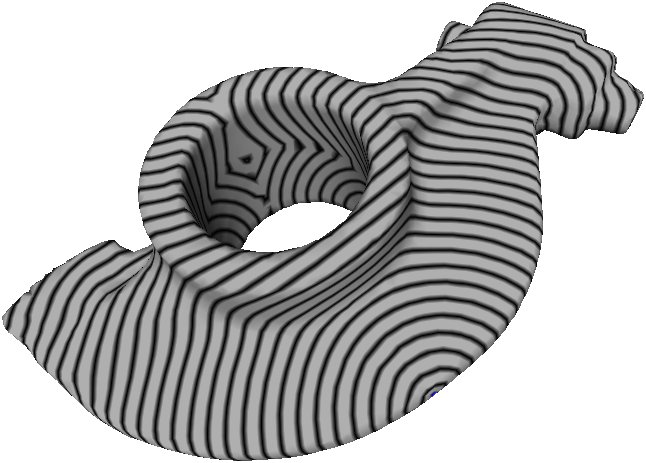
\includegraphics[width=0.9\columnwidth]{images/geodesic_rocket-arm.png}}
	\caption{Geodesic distance radius from a starting point on genus 1 rocket arm model. At the hole, we can see some sharp pattern which can be recognize as geodesic path came from different directions.}
	\label{fig:geodesic rocket arm}
\end{figure}



\section{\uppercase{Related Works}}
\noindent From previous researches in topological converting topic in the past few years, there was a novel study the problem of cutting a topological surface into the disk efficiently by \cite{Erickson:2002:OCS:513400.513430}. They have proposed a cutting method which has some elegant theoretical guarantees but is complex to implement. It finds the shortest loop path connecting a vertex to the vertex itself by using a front propagation technique, and then tests to see if the considering loop path reduces the surface genus or simply cut the surface into two pieces. The generation of minimal length cuts that convert a high genus surface into a topological disk is a NP-hard problem. The method is a brute force approach which consumes a lot of time. it has approximation of the shortest cut graph in $O(g^2 n \log n)$. In more study from \cite{Erickson:2005:GOH:1070432.1070581}, they studied about greedy homotopy basis and improvement speed in $O(n \log n)$
by using a straightforward application of Dijkstra's shortest path algorithm \cite{Dijkstra59anote}. 

One of important in efficiency is to compute non-trivial cycles on orientable surfaces. Non-trivial cycles mean non-contractible and non-separating cycles which guarantees cutting topological surface into disk. Recently, \cite{Kutz:2006:CSN:1137856.1137919} presents an algorithm that computes a shortest non-trivial cycles on orientable combinatorial surface of bounded genus in  $O(n \log n)$. The algorithm is based on universal-cover constructions to find short cycles.

There are studies that trying to define cut graph by properties of surfaces. Study from \cite{Patane:2007:FCB:1224804.1224947} presents an algorithm that build up the cut graph on the iso-contours from Reeb graph which codes in a combinatorial structure the topology of a given surface $M$ and connect loops together. Study from \cite{Jin:2013:CSH:2396897.2396971}, presents algorithm to compute the shortest homotopic loop with negative Euler characteristic based on the surface hyperbolic uniformization metric.

\subsection{Manuscript Setup}

\noindent The template is composed by a set of 7 files, in the
following 2 groups:\\
\noindent {\bf Group 1.} To format your paper you will need to copy
into your working directory, but NOT edit, the following 4 files:
\begin{verbatim}
  - apalike.bst
  - apalike.sty
  - article.cls
  - scitepress.sty
\end{verbatim}

\noindent {\bf Group 2.} Additionally, you may wish to copy and edit
the following 3 example files:
\begin{verbatim}
  - example.bib
  - example.tex
  - scitepress.eps
\end{verbatim}


\subsection{Page Setup}

The paper size must be set to A4 (210x297 mm). The document
margins must be the following:

\begin{itemize}
    \item Top: 3,3 cm;
    \item Bottom: 4,2 cm;
    \item Left: 2,6 cm;
    \item Right: 2,6 cm.
\end{itemize}

It is advisable to keep all the given values because any text or
material outside the aforementioned margins will not be printed.

\subsection{First Section}

This section must be in one column.

\vfill
\subsubsection{Title and Subtitle}

Use the command \textit{$\backslash$title} and follow the given structure in "example.tex". The title and subtitle must be with initial letters
capitalized (titlecased). If no subtitle is required, please remove the corresponding \textit{$\backslash$subtitle} command. In the title or subtitle, words like "is", "or", "then", etc. should not be capitalized unless they are the first word of the subtitle. No formulas or special characters of any form or language are allowed in the title or subtitle.

\subsubsection{Authors and Affiliations}

Use the command \textit{$\backslash$author} and follow the given structure in "example.tex".

\subsubsection{Keywords}

Use the command \textit{$\backslash$keywords} and follow the given structure in "example.tex". Each paper must have at least one keyword. If more than one is specified, please use a comma as a separator. The sentence must end with a period.

\subsubsection{Abstract}

Use the command \textit{$\backslash$abstract} and follow the given structure in "example.tex".
Each paper must have an abstract up to 200 words. The sentence
must end with a period.

\subsection{Second Section}

Files "example.tex" and "example.bib" show how to create a paper
with a corresponding list of references.

This section must be in two columns.

Each column must be 7,5-centimeter wide with a column spacing
of 0,8-centimeter.

The section text must be set to 10-point.

Section, subsection and sub-subsection first paragraph should not
have the first line indent.

To remove the paragraph indentation (only necessary for the
sections), use the command \textit{$\backslash$noindent} before the
paragraph first word.

If you use other style files (.sty) you MUST include them in the
final manuscript zip file.

\subsubsection{Section Titles}

The heading of a section title should be in all-capitals.

Example: \textit{$\backslash$section\{FIRST TITLE\}}

\vfill
\subsubsection{Subsection Titles}

The heading of a subsection title must be with initial letters
capitalized (titlecased).

Words like "is", "or", "then", etc. should not be capitalized unless
they are the first word of the subsection title.

Example: \textit{$\backslash$subsection\{First Subtitle\}}

\subsubsection{Sub-Subsection Titles}

The heading of a sub subsection title should be with initial letters
capitalized (titlecased).

Words like "is", "or", "then", etc should not be capitalized unless
they are the first word of the sub subsection title.

Example: \textit{$\backslash$subsubsection\{First Subsubtitle\}}

\subsubsection{Tables}

Tables must appear inside the designated margins or they may span
the two columns.

Tables in two columns must be positioned at the top or bottom of the
page within the given margins. To span a table in two columns please add an asterisk (*) to the table \textit{begin} and \textit{end} command.

Example: \textit{$\backslash$begin\{table*\}}

\hspace*{1.5cm}\textit{$\backslash$end\{table*\}}\\

Tables should be centered and should always have a caption
positioned above it. The font size to use is 9-point. No bold or
italic font style should be used.

The final sentence of a caption should end with a period.

\begin{table}[h]
\caption{This caption has one line so it is
centered.}\label{tab:example1} \centering
\begin{tabular}{|c|c|}
  \hline
  Example column 1 & Example column 2 \\
  \hline
  Example text 1 & Example text 2 \\
  \hline
\end{tabular}
\end{table}

\begin{table}[h]
\caption{This caption has more than one line so it has to be
justified.}\label{tab:example2} \centering
\begin{tabular}{|c|c|}
  \hline
  Example column 1 & Example column 2 \\
  \hline
  Example text 1 & Example text 2 \\
  \hline
\end{tabular}
\end{table}

Please note that the word "Table" is spelled out.


\subsubsection{Figures}

Please produce your figures electronically, and integrate them into
your document and zip file.

Check that in line drawings, lines are not interrupted and have a
constant width. Grids and details within the figures must be clearly
readable and may not be written one on top of the other.

Figure resolution should be at least 300 dpi.

Figures must appear inside the designated margins or they may span
the two columns.

Figures in two columns must be positioned at the top or bottom of
the page within the given margins. To span a figure in two columns please add an asterisk (*) to the figure \textit{begin} and \textit{end} command.

Example: \textit{$\backslash$begin\{figure*\}}

\hspace*{1.5cm}\textit{$\backslash$end\{figure*\}}

Figures should be centered and should always have a caption
positioned under it. The font size to use is 9-point. No bold or
italic font style should be used.

\begin{figure}[!h]
  %\vspace{-0.2cm}
  \centering
   {
\epsfig{file = SCITEPRESS.eps, width = 5.5cm}}
  \caption{This caption has one line so it is centered.}
  \label{fig:example1}
 \end{figure}

\begin{figure}[!h]
  \vspace{-0.2cm}
  \centering
   {
\epsfig{file = SCITEPRESS.eps, width = 5.5cm}}
  \caption{This caption has more than one line so it has to be justified.}
  \label{fig:example2}
  \vspace{-0.1cm}
\end{figure}

The final sentence of a caption should end with a period.



Please note that the word "Figure" is spelled out.

\subsubsection{Equations}

Equations should be placed on a separate line, numbered and
centered.\\The numbers accorded to equations should appear in
consecutive order inside each section or within the contribution,
with the number enclosed in brackets and justified to the right,
starting with the number 1.

Example:

\begin{equation}\label{eq1}
    a=b+c
\end{equation}

\subsubsection{Program Code}\label{subsubsec:program_code}

Program listing or program commands in text should be set in
typewriter form such as Courier New.

Example of a Computer Program in Pascal:

\begin{small}
\begin{verbatim}
 Begin
     Writeln('Hello World!!');
 End.
\end{verbatim}
\end{small}


The text must be aligned to the left and in 9-point type.

\vfill
\subsubsection{Reference Text and Citations}

References and citations should follow the Harvard (Author, date)
System Convention (see the References section in the compiled
manuscript). As example you may consider the citation
\cite{Smith98}. Besides that, all references should be cited in the
text. No numbers with or without brackets should be used to list the
references.

References should be set to 9-point. Citations should be 10-point
font size.

You may check the structure of "example.bib" before constructing the
references.

For more instructions about the references and citations usage
please see the appropriate link at the conference website.

\section{\uppercase{Copyright Form}}

\noindent For the mutual benefit and protection of Authors and
Publishers, it is necessary that Authors provide formal written
Consent to Publish and Transfer of Copyright before publication of
the Book. The signed Consent ensures that the publisher has the
Author's authorization to publish the Contribution.

The copyright form is located on the authors' reserved area.

The printed form should be completed and signed by one author on
behalf of all the other authors, and uploaded through the authors' reserved area. Alternatively, you can send it to the secretariat by e-mail or fax.

\section{\uppercase{Conclusions}}
\label{sec:conclusion}

\noindent Please note that ONLY the files required to compile your paper should be submitted. Previous versions or examples MUST be removed from the compilation directory before submission.

We hope you find the information in this template useful in the preparation of your submission.

\section*{\uppercase{Acknowledgements}}

\noindent If any, should be placed before the references section
without numbering. To do so please use the following command:
\textit{$\backslash$section*\{ACKNOWLEDGEMENTS\}}


\vfill
\bibliographystyle{apalike}
{\small
\bibliography{genus_cutting}}


\section*{\uppercase{Appendix}}

\noindent If any, the appendix should appear directly after the
references without numbering, and not on a new page. To do so please use the following command:
\textit{$\backslash$section*\{APPENDIX\}}

\vfill
\end{document}

